\documentclass[11pt, oneside]{article}  
\usepackage[margin=0.5in]{geometry} % Margins
\usepackage[ampersand]{easylist} % Bullets for lists
\usepackage[bottom]{footmisc}  % Glue footnotes to bottom
\usepackage{graphicx}
\usepackage{float}
\graphicspath{ {imgs/} }


\title{Algorithms and Complexity\\UCLA-CS180-S18}
\author{Quentin Truong\\Taught by Professor Meka}
\date{Spring 2018}


\begin{document}
\maketitle
\tableofcontents
\pagenumbering{arabic}
\clearpage


%========================================================
\section{Algorithm Design: Ch5: Divide and Conquer}
\subsection{Introduction}
	\begin{easylist}  
	\ListProperties(Hide=100, Hang=true, Progressive=4ex, Style*=--\ , Style2*=$\bullet\ $)
        & Divide and conquer
        && Class of algorithmic techniques in which one breaks input into several parts, solves subproblems recursively, and recombines into overall solution
        & Analyze running time
        && Generally will use recurrence relations
        && For divide and conquer problems, the brute force solution is typically polynomial; we are trying for a lower polynomial
	\end{easylist}

\subsection{A First Recurrence: The Mergesort Algorithm}
    \begin{easylist}  
    \ListProperties(Hide=100, Hang=true, Progressive=4ex, Style*=--\ , Style2*=$\bullet\ $)
        & Mergesort
        && Sort list of numbers by dividing into two equal halves, solving each half recursively, and recombining solutions
        && T(n) $\le$ 2T(n/2) + O(n)
        && Ignore ceiling and floor issues for odd numbers, b/c not actually impactful
        & Approaches to Solving Recurrences
        && Unrolling the recurrence into a graph allows us to see how many operations are performed at each level
        &&& Identify the pattern, and sum over all levels
        && Substituting a solution into the recurrence
        &&& Requires a guess
        && Partial substitution can determine the constants
        &&& Useful for determining exact constants if we know the general form of the solution
    \end{easylist}

\subsection{Further Recurrence Relations}
    \begin{easylist}  
    \ListProperties(Hide=100, Hang=true, Progressive=4ex, Style*=--\ , Style2*=$\bullet\ $)
        & 5.3 T(n) $\le$ qT(n/2) + cn
        & 5.4 Any function T() satisfiyng 5.3 with q \textgreater 2 is bounded by O($n^{\log_2q}$)
        & 5.5 Any function T() satisfying 5.3 with q=1 is bounded by O(n)
        & 5.6 T(n) $\le$ 2T(n/2) + cn$^2$
    \end{easylist}

\subsection{Counting Inversions}
    \begin{easylist}  
    \ListProperties(Hide=100, Hang=true, Progressive=4ex, Style*=--\ , Style2*=$\bullet\ $)
        \begin{figure}[H]
            \centering
            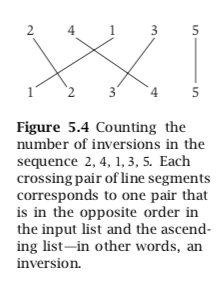
\includegraphics[scale=.6]{./imgs/count_inversions.png}
        \end{figure}
        & Application of Counting Inversions
        && Analysis of rankings
        &&& Collaborative filtering, to match preferences to those of other people on the Internet
        &&& Recommend things according to what other similar people like
        && Meta-search tools
        &&& Execute same query on different search engines
        &&& Measure how "out of order" the different orderings are
        && Generally
        &&& Given a sequence of distinct numbers, measure how far the list is from being in ascending order
        &&& Number should increase as more scrambled
        & More formal definition of Counting Inversions
        && Count the number of indices i \textless j which form an inversion, a$_i$ \textgreater a$_j$
        & Algorithm
        && Divide list in two halves, recursively sort and count inversions for each
        && To recombine two halves, take min of each sorted half
        && If take min from first half, no inversions are added
        && If take min from the second half, then add the number of remaining elements from the first half to the inversion count
    \end{easylist}

\subsection{Finding the Closest Pair of Points}
    \begin{easylist}  
    \ListProperties(Hide=100, Hang=true, Progressive=4ex, Style*=--\ , Style2*=$\bullet\ $)
        & 1D Algorithm
        && Sort; min must be adjacent to each other, so traverse
        & 2D Algorithm
        && P$_x$ are the points sorted with respect to x
        && P$_y$ are the points sorted with respect to y
        && L is the line dividing P$_x$ in half
        && Q are first half of points in P$_x$
        && R are second half of points in P$_x$
        && Recursively determine closest pair of points in Q; then in R
        && $\delta$ = min(d($q_0^*,q_1^*$), d($r_0^*,r_1^*$))
        && If there exists q $\in$ Q and r $\in$ R for which d(q, r) \textless $\delta$, then each of q and r lies within a distance of $\delta$ of L
        && If s, s$^\prime$ have d(s, s$^\prime$), then s and s$^\prime$ are within 15 positions of each other in the sorted S$_y$
        &&& Each box has sidelength ($\delta$/2), and at most one point (b/c if had more than one point, $delta$ would be different)
        &&& 16 boxes leads to 16 possible positions
        &&& Can reduce down to 5 possible positions using packing arguments
        &&& Linear time to try/fail find a position in S
        && Bruteforce for $P \le 3$
        && Satisfies recurence found in 5.1 to achieve O(nlogn)
    \end{easylist}

\subsection{Integer Multiplication}
    \begin{easylist}  
    \ListProperties(Hide=100, Hang=true, Progressive=4ex, Style*=--\ , Style2*=$\bullet\ $)
        & Multiplication
        && Adding up partial products works the same in base-10 as in base-2
        & Karatsuba's Algorithm
        && Based on breaking up partial sums
        && $xy = (x_1 * 2^{n/2} + x_0)(y_1 * 2^{n/2} + y_0$
        && $ = x_1y_1 * 2^n + (x_1y_0 + x_0y_1) * 2^{n/2} + x_0y_0$
        && This achieves T(n) $\le$ 4T(n/2) + cn = O(n$^2$)
        && $(x_1 + x_0)(y_1 + y_0) = x_1y_1 + x_1y_0 + x_0y_1 + x_0y_0$
        && Subtract away $x_1y_1$ and $x_0y_0$
        & Analysis
        && T(N) $\le$ 3T(n/2) + O(n)
        && O($n^{log_23}$)
    \end{easylist}

\subsection{Convolutions and the Fast Fourier Transform}
    \begin{easylist}  
    \ListProperties(Hide=100, Hang=true, Progressive=4ex, Style*=--\ , Style2*=$\bullet\ $)
        & Convolution
        && Take two vectors of length n and produce a vector of 2n - 1 coordinates
        && $\sum_{(i,j):i+j=k;i,j<n}a_ib_j$
        && Many applications, especially in signal processing
        & Fast Fourier Transform
        && Can calculate convoution in nlogn
        && Product of polynomials is equivalent to convolution
        && Reconstruct C from values on the (2n)$^{th}$ roots of complex roots of unity
        && Coefficients of C are coordinates of convolution vector
    \end{easylist}
\clearpage
%========================================================

%========================================================
\section{Ch3: Graphs}
\subsection{Basic Definitions and Applications}
    \begin{easylist}  
    \ListProperties(Hide=100, Hang=true, Progressive=4ex, Style*=--\ , Style2*=$\bullet\ $)
        & Graph is a collection V of nodes and collection E of edges
        & Undirected Graph
        && Edge is two-element subset of V
        & Directed Graph
        && Edge is an ordered pair of two vertices
        & Applications
        && Transportation networks: airplanes and trains
        && Communication networks: wired and wireless
        && Information networks: WWW as directed graph
        && Social networks: used to study interactions among people, etc
        && Dependency networks: university course offerings with prereqs, food web, software modules
        & Paths and Connectivity
        && Path in undirected graph is sequence of consecutive nodes joined by edges
        && Path is simpe if all vertices are distinct
        && Cycle is sequence of 3 or more vertices where first and last vertex are the same
        && Undirected graph is connected if there is a path between all pairs of nodes
        && Directed graph is strongly connected if for all nodes u and v, there is path uv and vu
        && Distance between nodes is minimum number of edges
        && Trees are undirected, connected graphs without cycles
        &&& Orient edges away from each other, such that nodes are descendants of ancestors
        &&& (3.1) Every n-node tree has exactly n-1 edges
        && Rooted trees show a hierarchy
        & (3.2) Let G be undirected graph on n nodes. Any two implies third
        && G is connected
        && G does not contain a cycle
        && G has n-1 edges
    \end{easylist}

\subsection{Graph Connectivity and Graph Traversal}
    \begin{easylist}  
    \ListProperties(Hide=100, Hang=true, Progressive=4ex, Style*=--\ , Style2*=$\bullet\ $)
        & S-T Connectivity (Maze-solving)
        && Use BFS and DFS
        & Breadth-First Search (BFS)
        && (3.3) For each j $\ge$ 1, layer L$_j$ produced by BFS consists of all nodes at distance exactly j from s. There is a path from s to t iff t appears in some layer
        && (3.4) Nodes X and Y in BFS tree in layers L$_i$ and L$_j$ are connected by an edge, then i and j differ by at most 1
        & Exploring a Connected Component
        && BFS discovers the set of reachable nodes
        && Could discover this set in many ways
        & Depth-First Search (DFS) (Maze-exploration)
        && Explore as deeply as possible, retreat only when necessary 
        && Maintain global knowledge of which nodes have been explored
        & Set of all Connected Components
        && (3.8) For any two nodes, their connected components are either identical or disjoint
    \end{easylist}

\subsection{Implementing Graph Traversal Using Queues and Stacks}
    \begin{easylist}  
    \ListProperties(Hide=100, Hang=true, Progressive=4ex, Style*=--\ , Style2*=$\bullet\ $)
        & Representing Graphs
        && Adjacency Matrix
        &&& n x n matrix where A[u, v] is 1 if contains edge
        &&& $\Theta$(n$^2$) space
        &&& $\Theta$(n) time to find incident edges
        && Adjacency List
        &&& Reecord for each node v, containing list of nodes to which v has edges
        &&& Total length of al lists is 2m = O(m)
        &&& Much better for sparse
        &&& O(m+n) space where m is edges n is nodes
        & BFS - Queue
        & DFS - Stack
        & Finding Set of All Connected Components
        && BFS/DFS a node, repeat on unconnnected nodes until find all groups
    \end{easylist}

\subsection{Testing Bipartiteness: Application of BFS}
    \begin{easylist}  
    \ListProperties(Hide=100, Hang=true, Progressive=4ex, Style*=--\ , Style2*=$\bullet\ $)
        & (3.14) Bipartite graph cannot contain odd cycle
        & Red-Blue
        && Color node red, BFS, color all those blue, BFS, swap back to red
        && Once all colored, scan all edges, check for edges with same colors on both sides of edge
    \end{easylist}

\subsection{Connectivity in Directed Graphs}
    \begin{easylist}  
    \ListProperties(Hide=100, Hang=true, Progressive=4ex, Style*=--\ , Style2*=$\bullet\ $)
        & Directed Graphs
        && Adjacency list has two list
        &&& Nodes to which it has edges
        &&& Nodes from which it has edges
        & Graph Search Algorithms
        && BFS/DFS will traverse set of nodes to which starting node is connected to
        && If want set of nodes with paths to s (not set of nodes to which s has paths), reverse direction of every edge, then run BFS/DFS from this new s
        & Strong Connectivity
        && For every two nodes, there is path from u to v and v to u
        & Mutually Reachable
        && Path from u to v and v to u
        & (3.17) For any two nodes, their strongly connected component is either identical or disjoint
    \end{easylist}

\subsection{Directed Acyclic Graphs and Topological Ordering}
    \begin{easylist}  
    \ListProperties(Hide=100, Hang=true, Progressive=4ex, Style*=--\ , Style2*=$\bullet\ $)
        & Undirected Graph without cycles
        && Each connected component is a tree
        & Directed Acylic Graphs
        && Used often as graph for dependencies 
        & Topological Ordering
        && Every edge points forward in the ordering
        && Ordering of nodes, such that for every edge (v$_i$, v$_j$), we have i \textless j
        && Topological ordering can provide immediate visual proof of no cycles
        && Topological ordering implies DAG
        && DAG implies topological ordering
        & Computing Topological Ordering
        && Find node with no incoming edges, place it first
        && Delete that node
        && Recursively compute topological ordering for rest of graph
        && Append deleted node to front of remaining topological ordeing
        && Complexity Analysis
        &&& O(n$^2$) - Trivially search
        &&& O(m+n) - If track number of incoming edges for each node and set of nodes without incoming edges
    \end{easylist}
\clearpage
%========================================================

%========================================================
\section{Ch3: Graphs}
\subsection{Basic Definitions and Applications}
    \begin{easylist}  
    \ListProperties(Hide=100, Hang=true, Progressive=4ex, Style*=--\ , Style2*=$\bullet\ $)
        &
    \end{easylist}
\clearpage
%========================================================

\end{document}
